\documentclass[a4paper,10pt,ngerman,captions=figureheading]{scrartcl}
\usepackage{babel}
\usepackage[T1]{fontenc}
\usepackage[utf8x]{inputenc}
\usepackage[a4paper,margin=2.5cm,footskip=0.5cm]{geometry}

% todo: check TeilnahmeId
\newcommand{\Aufgabe}{Aufgabe 3: Eisbudendilemma}
\newcommand{\TeilnahmeId}{56860}
\newcommand{\Name}{Christopher Besch}


% header and footer
\usepackage{scrlayer-scrpage, lastpage}
\setkomafont{pageheadfoot}{\large\textrm}
\lohead{\Aufgabe}
\rohead{Teilnahme-ID: \TeilnahmeId}
\cfoot*{\thepage{}/\pageref{LastPage}}

% title position
\usepackage{titling}
\setlength{\droptitle}{-1.0cm}

% for math commands and symbols
\usepackage{amsmath}
\usepackage{amssymb}

% for images
\usepackage{graphicx}
\graphicspath{{images/}}
\usepackage{subcaption}

% for tables
\usepackage{tabularx}
\usepackage{booktabs}
\usepackage{ltablex}

% for algorithms
\usepackage{algpseudocode}

% for indented block
\usepackage{scrextend}

% for source code
\usepackage{listings}
\usepackage{color}
\definecolor{mygreen}{rgb}{0,0.6,0}
\definecolor{mygray}{rgb}{0.5,0.5,0.5}
\definecolor{mymauve}{rgb}{0.58,0,0.82}
\lstset{
  keywordstyle=\color{blue},commentstyle=\color{mygreen},
  stringstyle=\color{mymauve},rulecolor=\color{black},
  basicstyle=\footnotesize\ttfamily,numberstyle=\tiny\color{mygray},
  captionpos=b, % sets the caption-position to bottom
  keepspaces=true, % keeps spaces in text
  numbers=left, numbersep=5pt, showspaces=false,showstringspaces=true,
  showtabs=false, stepnumber=2, tabsize=2, title=\lstname
}
\lstdefinelanguage{JavaScript}{ % JavaScript is the only non-predefined language
  keywords={break, case, catch, continue, debugger, default, delete, do, else, finally, for, function, if, in, instanceof, new, return, switch, this, throw, try, typeof, var, void, while, with},
  morecomment=[l]{//},
  morecomment=[s]{/*}{*/},
  morestring=[b]',
  morestring=[b]",
  sensitive=true
}

% these packages must be loaded last
\usepackage{hyperref}
\usepackage{cleveref}

% c++ source code setup
\lstset{
    language=C++,
    basicstyle=\small\sffamily,
    numbers=left,
    numberstyle=\tiny,
    frame=tb,
    tabsize=4,
    columns=fixed,
    showstringspaces=false,
    showtabs=false,
    keepspaces,
    commentstyle=\color{red},
    keywordstyle=\color{blue}
}

\newcommand{\imageWidth}{0.3\linewidth}

% title
\title{\textbf{\Huge\Aufgabe}}
\author{\LARGE Teilnahme-ID: \LARGE \TeilnahmeId \\\\
	    \LARGE Bearbeiter/-in dieser Aufgabe: \\ 
	    \LARGE \Name\\\\}
\date{\LARGE\today}

\begin{document}

\maketitle
\tableofcontents

\vspace{0.5cm}

\section{Lösungsidee}
% Die Idee der Lösung sollte hieraus vollkommen ersichtlich werden, ohne dass auf die eigentliche Implementierung Bezug genommen wird.
Das Ziel ist es, ein Arrangement bestehend aus drei Positionen für Eisdielen zu generieren, das in einer Abstimmung durch kein anderes Arrangement abgelöst werden kann.
Diese Arrangements werden \emph{stabil} genannt.
Hierzu darf die \emph{Eisdielendistanz}, die Strecke zwischen einem beliebigen Haus und der nächsten Eisdiele, von nicht mehr als der Hälfte der Hauser durch ein anderes Arrangement verkürzt werden.
Wäre dies der Fall, würde die Ablösung mehr Ja- als Nein-Stimmen erhalten.

Hieraus geht hervor, dass für eine optimale Lösung alle möglichen Arrangements auf Stabilität überprüft werden müssen.
Diese werden \emph{Test-Arrangement} genannt.
Um die Stabilität zu bestimmen, muss das Test-Arrangement mit allen möglichen anderen Arrangements (\emph{Check-Arrangements} genannt) verglichen werden.
Wenn auch nur ein einziges Check-Arrangement gefunden wird, das mehr Ja- als Nein-Stimmen erhält, ist das getestete Test-Arrangement instabil.
Es lässt sich leicht erkennen, dass dieser Algorithmus, der Durchgang aller möglichen Test-Arrangements, mit einer Laufzeit von $O(n^6)$ nicht verwendbar ist.
Allerdings entspricht er einer 1:1 Umsetzung der Bedingungen und produziert damit garantiert alle korrekten Ergebnisse und alle Ergebnisse, die er generiert, sind korrekt.

\subsection{Ein Wort über die Graphiken}
Alle in dieser Dokumentation verwendeten Darstellungen verwenden einheitliche Symbole:
\begin{itemize}
    \item Der See ist als schwarzer Kreis dargestellt.
    \item Die Häuser sind verschieden gefärbte Rechtecke, deren Adresse außerhalb des Kreises stehen:
          \begin{itemize}
              \item Rot: Das Haus stimmt gegen eine Verlegung der Eisdielen.
              \item Grün: Es stimmt für eine Verlegung.
              \item Andere Farben werden verwendet, um bestimmte Häuser hervorzuheben.
          \end{itemize}
    \item Die Adressen sind aufsteigend im Uhrzeigersinn angeordnet.
          Adresse $0$, die Dorfkirche, befindet sich oben.
    \item Blaue Kreuze stellen die Positionen des Test-Arrangements dar und
    \item blaue Kreise die des Check-Arrangements.
          In beiden Fällen stehen die Adressen innerhalb des Kreises.
\end{itemize}

\subsection{Sortierung der Arrangements}
\label{sec:Sortierung_der_Arrangements}
Als Versuch der Optimierung werden bevor sie getestet werden alle Arrangement sortiert.
Hierzu wird für jedes mögliche Arrangement ein Score berechnet.
Dieser entspricht der durchschnittlichen Eisdielendistanz aller Häuser.
Nun stellt sich heraus, dass stabile Arrangements auch die niedrigsten Scores aller Arrangements aufweisen.
Dies lässt sich damit erklären, dass je kleiner die Eisdielendistanz eines Hauses in einem Test-Arrangement ist, desto weniger Check-Arrangements existieren, die eine noch geringere Eisdielendistanz für das Haus generieren.
Wenn die Eisdielendistanz beispielsweise $0$ beträgt, existiert kein einziges Check-Arrangement, dem dieses Haus eine Ja-Stimme geben würde, da eine geringere Eisdielendistanz nicht möglich ist und ein Haus bei gleichbleibender Eisdielendistanz immer gegen eine Verlegung stimmt.
Dies ist in \autoref{fig:01_hapy_house} gezeigt.

\begin{figure}[h!t]
    \centering
    \caption{Das einzige Haus ist zufrieden mit der einzigen Eisdiele und lehnt jegliche Veränderung ab. Die Eisdielendistanz beträgt $0$.}
    \label{fig:01_hapy_house}
    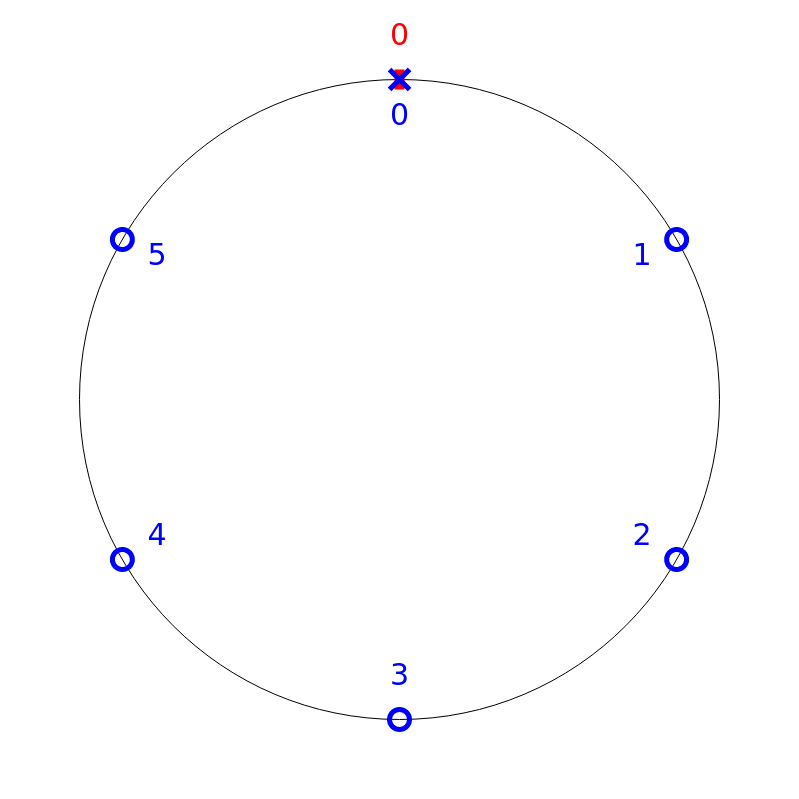
\includegraphics[width=\imageWidth]{01_happy_house.png}
\end{figure}

Wenn die Eisdielendistanz dem maximalen Wert, dem halben Umfang des Sees, entspricht, stimmt es für alle Check-Arrangements (\autoref{fig:02_unhappy_house}), abgesehen von denen, die die Eisdielendistanz nicht verändern (\autoref{fig:03_slightly_happy_house}).

\begin{figure}[h!t]
    \centering
    \caption{Unzufriedene Häuser}
    \begin{subfigure}[t]{\imageWidth}
        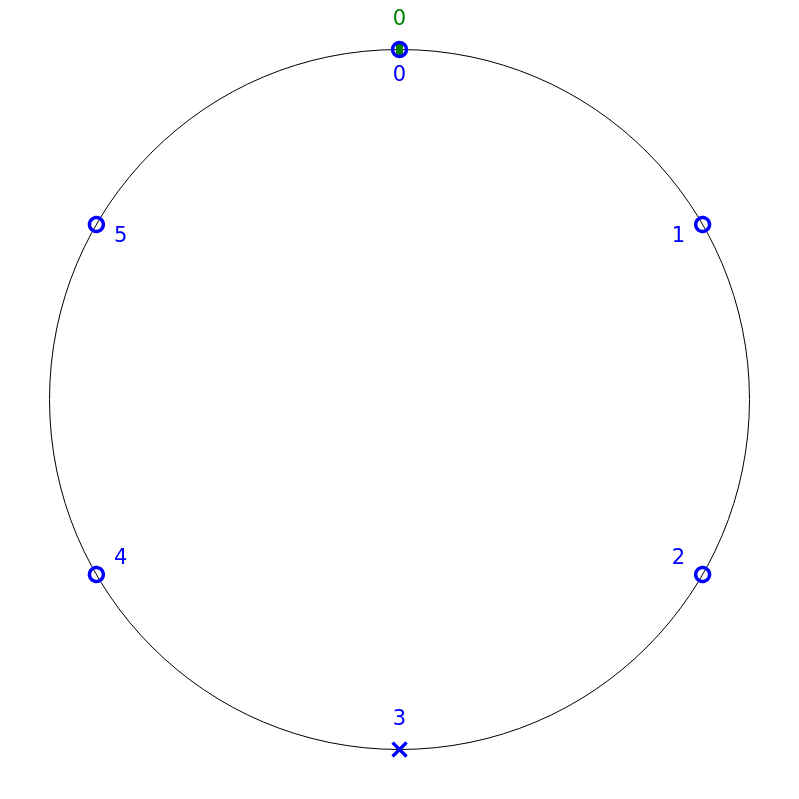
\includegraphics[width=\linewidth]{02_unhappy_house.png}
        \caption{Das Haus ist maximal unzufrieden, weshalb es für fast jede Verlegung stimmt. Jeder Kreis repräsentiert eine anderes Check-Arrangement, die alle von dem Haus angenommen werden.}
        \label{fig:02_unhappy_house}
    \end{subfigure}
    \begin{subfigure}[t]{\imageWidth}
        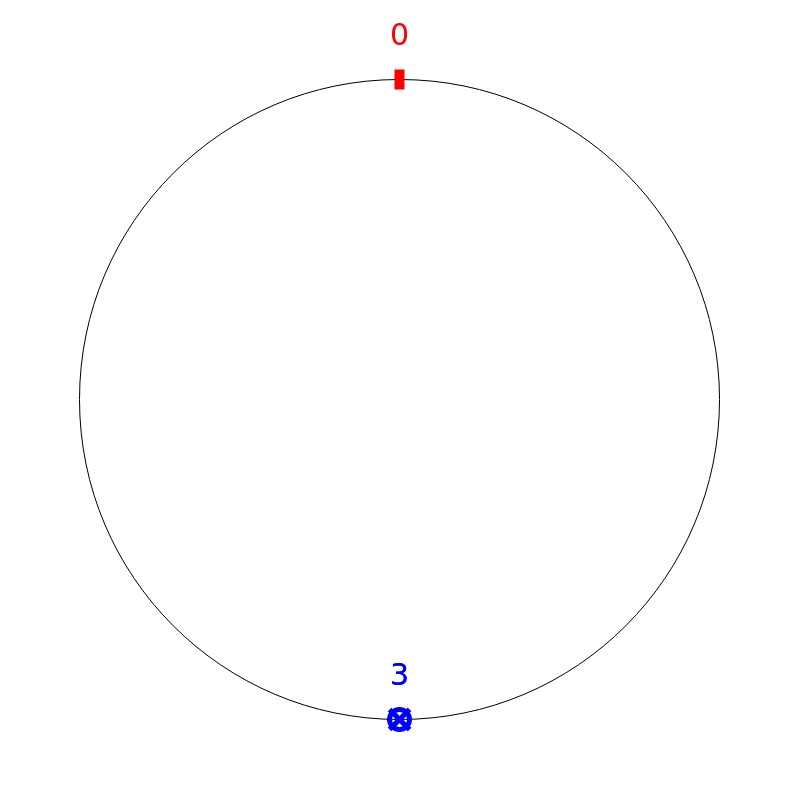
\includegraphics[width=\linewidth]{03_slightly_happy_house.png}
        \caption{Dies ist der einzige Fall, in dem das Haus trotz seiner extremen Unzufriedenheit gegen eine Verlegung stimmt.}
        \label{fig:03_slightly_happy_house}
    \end{subfigure}
\end{figure}

Die durchschnittliche Eisdielendistanz lässt sich dementsprechend als \glqq Zufriedenheitsgrad\grqq{} des Dorfes interpretieren.
Je höher er ist, desto unwahrscheinlicher wird eine Verlegung durchgesetzt.

Allerdings muss dieser Wert nicht zwangsweise mit der Stabilität eines Arrangements übereinstimmen, was beispielsweise in \autoref{fig:04_broken_example} gezeigt wird.

\begin{figure}[h!t]
    \centering
    \caption{Trotz der für dieses Beispiel, \textit{eisbuden3.txt}, minimalen durchschnittlichen Eisdielendistanz von $3,3125$ stimmen mehr Häuser für eine Verlegung.}
    \label{fig:04_broken_example}
    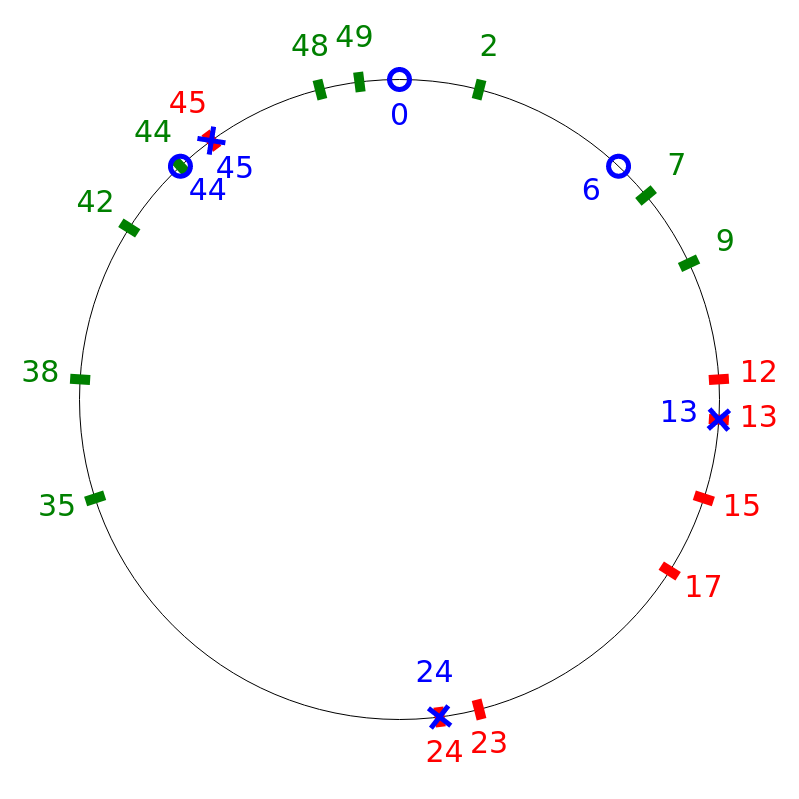
\includegraphics[width=\imageWidth]{04_broken_example.png}
\end{figure}

Hieraus geht hervor, dass die durchschnittliche Eisdielendistanz nur eine Näherungslösung liefert.
Trotzdem kann sie zur Generierung eines Satzes an Test-Arrangements, den $x$ Arrangements mit der geringsten durchschnittlichen Eisdielendistanz, verwendet werden, die anschließend von dem bereits genannten Algorithmus auf Stabilität überprüft werden.

\subsection{Bestimmung der Stabilität}
\label{sec:Bestimmung_der_Stabilität}
Um die Stabilität eines Test-Arrangements zu berechnen, müssen alle möglichen Check-Arrangements durchgegangen werden.
Es wird nur ein einziges Check-Arrangement gesucht, das das Test-Arrangement schlagen kann.
Daher können zwei Optimierungen getroffen werden:
\begin{enumerate}
    \item Eisdielen sollten nicht übereinander liegen, da bei der Aufsplittung zweier Aufeinanderliegender die Eisdielendistanz keines Häuses vergrößert wird.
    \item Alle Dopplungen sind unnötig, da die Reihenfolge der Eisdielen für die Stimmen der Häuser irrelevant ist.
\end{enumerate}
Deshalb darf die Bedingung gelten, dass die Adresse der zweiten Eisdiele größer als die der ersten und kleiner als die der dritten ist.
Hieraus folgt, dass der See immer in drei Sektoren unterteilt ist, dessen Grenzen Check-Eisdielen sind (\autoref{fig:05_sectors}).

\begin{figure}[h!t]
    \centering
    \caption{Einteilung in Sektoren}
    \label{fig:05_sectors}
    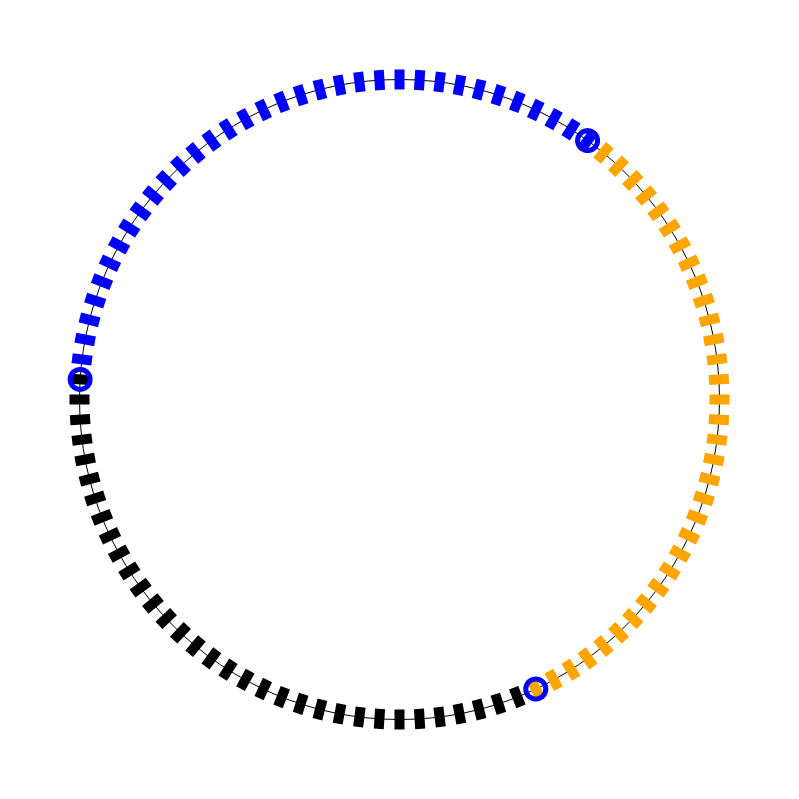
\includegraphics[width=\imageWidth]{05_sectors.png}
\end{figure}

\subsubsection{Auszählung der Stimmen}
\label{sec:Auszählung_der_Stimmen}
Es zeigt sich, dass die Stimme der Häuser innerhalb eines Sektors ausschließlich durch die Größe und Position des Sektors und die in dem Sektor befindlichen Eisdielen des Test-Arrangements determiniert sind.
\begin{itemize}
    \item Alle Test-Eisdielen außerhalb des Sektors sind von den Häusern immer weiter entfernt als die Ränder des Sektors, weshalb sich die Eisdielendistanz ohne Test-Eisdielen innerhalb des Sektors bei Verlegung immer verkürzen würde.
    \item Genauso ist für jedes Haus im Sektor eine der Sektorgrenzen immer die nächste Check-Eisdiele.
          Dementsprechend ist die Position der dritten Check-Eisdiele ebenfalls irrelevant. da immer nur die Eisdielendistanz betrachtet wird.
\end{itemize}
Aus diesen beiden Tatsachen geht hervor, dass ausschließlich die Ränder des Sektors und die sich im Sektor befindlichen Test-Eisdielen Einfluss auf die Stimme eines Hauses in dem Sektor haben.

\medskip
Nun wird die Verteilung der Ja- und Nein-Stimmen betrachtet.
In einem Sektor können sich keine (\autoref{fig:06_no_test_ice}) nur eine (\autoref{fig:07_one_test_ice}) oder mehrere Eisdielen (\autoref{fig:08_two_test_ice}) befinden.

\begin{figure}[h!t]
    \centering
    \caption{Test-Eisdielen Anordnung im Sektor}
    \begin{subfigure}[t]{\imageWidth}
        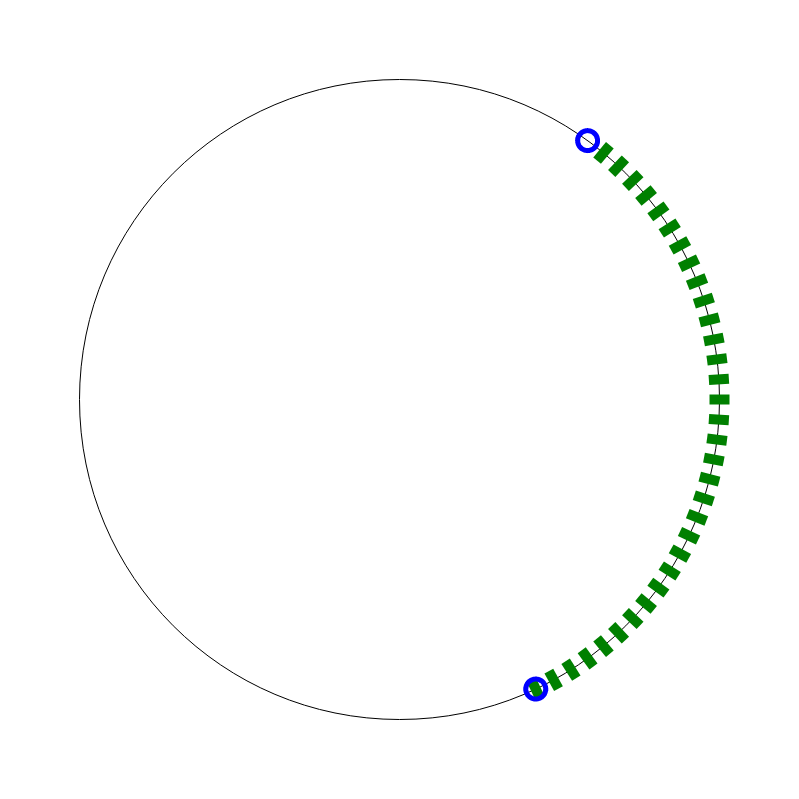
\includegraphics[width=\linewidth]{06_no_test_ice.png}
        \caption{Keine Test-Eisdiele}
        \label{fig:06_no_test_ice}
    \end{subfigure}
    \begin{subfigure}[t]{\imageWidth}
        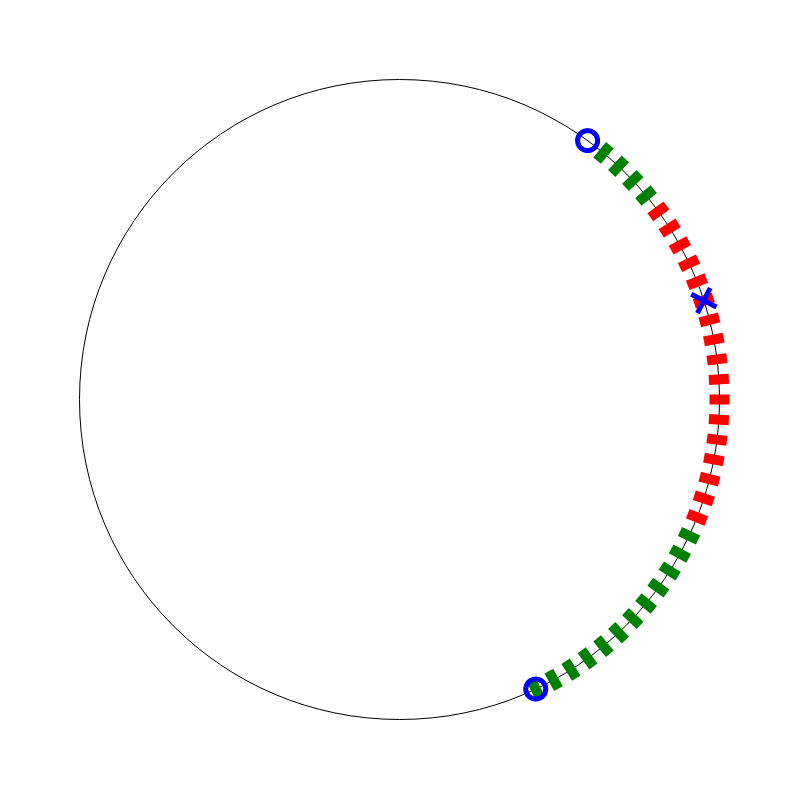
\includegraphics[width=\linewidth]{07_one_test_ice.png}
        \caption{Eine Test-Eisdiele}
        \label{fig:07_one_test_ice}
    \end{subfigure}
    \begin{subfigure}[t]{\imageWidth}
        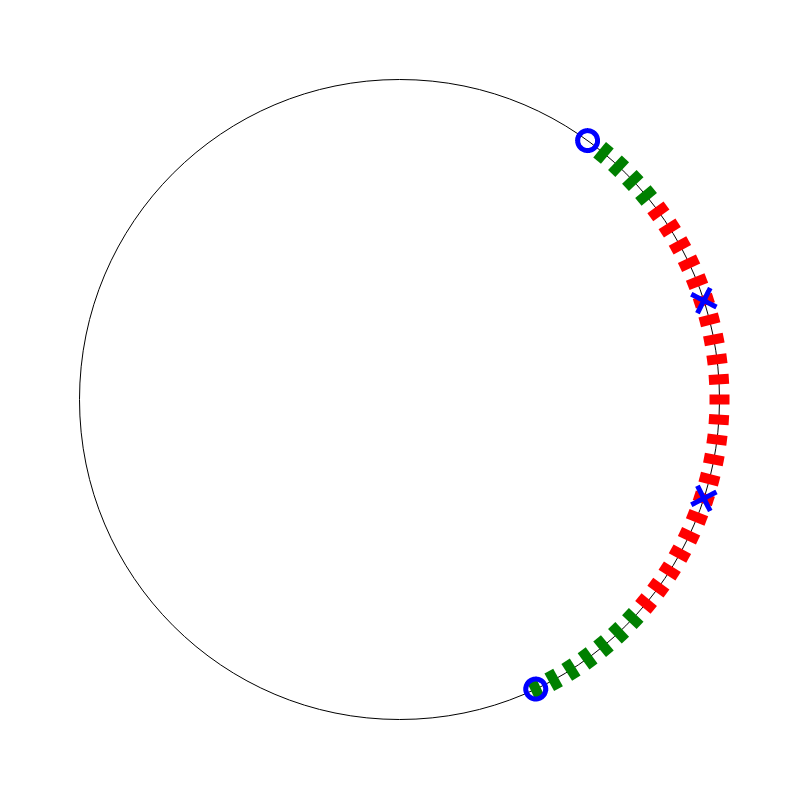
\includegraphics[width=\linewidth]{08_two_test_ice.png}
        \caption{Zwei oder mehr Test-Eisdielen (nur die Äußersten dargestellt)}
        \label{fig:08_two_test_ice}
    \end{subfigure}
\end{figure}

In dem letzten Fall, von mehr als einer Test-Eisdielenn im Sektor, müssen nur die äußersten betrachtet werden, da zwischen diesen beiden keine Check-Eisdiele stehen kann.
Dies geht aus der Definition eines Sektors hervor.
Somit stimmen immer alle Häuser zwischen diesen gegen eine Verlegung, unabhängig von der Menge an Test-Eisdielen.

Um die Anzahl an Nein- beziehungsweise Ja-stimmenden Häusern zu bestimmen, werden zwei verschiedene Methoden verwendet:
\begin{itemize}
    \item Wenn sich keine Test-Eisdiele in dem Sektor befindet, stimmen alle Häuser für eine Verlegung.
    \item In allen anderen Fällen befinden sich die einzigen Ja-stimmenden Häuser in den beiden Bereichen zwischen einem Rand und der nächsten Test-Eisdiele.
          Wenn diese Bereiche in der Mitte geteilt wird, befinden sich alle Ja-stimmenden Häuser in der Hälfte, die näher am Rand ist.
          Alle Nein-stimmenden Häuser liegen in der anderen Hälfte.
          Dies lässt sich gut in \autoref{fig:08_two_test_ice} erkennen.
          Bei einer ungeraden Anzahl an Adressen in diesem Bereich wird der Nein-stimmenden Hälfte eine Adresse mehr zugeteilt, da bei gleichbleibender Eisdielendistanz das Haus Nein stimmt.
\end{itemize}
Auf diese Weise können effizient die Bereiche berechnet werden, in denen alle sich befindlichen Häuser mit Nein stimmen.

\medskip
Um alle Positionen für die Check-Eisdielen durchzugehen, können zuerst zwei Positionen für die ersten beiden Eisdielen festgesetzt werden und daraufhin alle möglichen Positionen für die dritte Eisdiele verwendet werden, die die genannten Bedingungen erfüllt.
Die verschiedenen Optionen für die ersten beiden Check-Eisdielen müssen in einem übergeordneten Schritt durchgegangen werden.
Somit ist die Größe und Position des ersten Sektors bei vielen Durchläufen gleich.
Wenn bereits mindestenz die Hälfte der Häuser sich in diesem Sektor befinden und gegen eine Veränderung stimmen, ist das Check-Arrangement unfähig, das Test-Arrangement abzulösen.
Somit kann in diesem Fall die Suche nach Positionen für die dritte Check-Eisdiele übersprungen werden und die Wahl der ersten beiden Check-Eisdielen sofort geändert werden.

\section{Umsetzung}
% Hier wird kurz erläutert, wie die Lösungsidee im Programm tatsächlich umgesetzt wurde. Hier können auch Implementierungsdetails erwähnt werden.
Die Lösungsidee wird in C++ implementiert.
Der Übersichtlichkeit halber ist das Programm in drei Dateien unterteilt:
\begin{itemize}
    \item \textbf{main.cpp} liest die Eingabe und gibt die Ergebnisse aus,
    \item \textbf{utils.h} enthält verwendete Structs und generell anwendbare Funktionen und Makros und
    \item \textbf{calculate\_stable.h} enthält die eigentlichen Funktionen zur Bestimmung der stabilen Arrangements.
\end{itemize}
Die einzigen Command Line Parameter, die das Programm benötigt, sind:
\begin{enumerate}
    \item der Pfad der Eingabedatei,
    \item die optionale Angabe der auf Stabilität zu überprüfenden Arrangements und
    \item die optionale Angabe der Menge zu verwendender Threads.
\end{enumerate}

Je geringer die Menge an besten Arrangements ist, desto kürzer ist die Laufzeit.
Allerdings ist ein zu niedriger Wert problemtisch, da wie bereits in \autoref{fig:04_broken_example} gezeigt, die stabilen Arrangements nicht zwingendermaßen die geringste Eisdielendistanz aufweisen.
Wenn kein Wert angegeben wird, werde die $600$ besten Arrangements überprüft.
Dieser Wert ist eine gute Wahl für die Beispieldateien.

Die Menge an Threads sollte nie die Menge an besten Arrangements überschreiten und wird standartmäßig auf eben diese Menge gesetzt.
Dieser Wert erwies sich für die Beispieldateien mit einem AMD Ryzen 5 2600 auf Ubuntu als der mit der geringsten Laufzeit.

\subsection{Einlese der Eingabedatei}
\label{sec:Einlese_der_Eingabedatei}
Als erster Schritt wird in der Funktion \textbf{read\_file} die Eingabedatei gelesen.
Hierbei wird überprüft, ob die Eingabedatei dem gegebenen Format entspricht; wenn nicht wird das Programm abgebrochen.
Hierzu wird ein Makro \textbf{raise\_error()} verwendet, das die Ausführung des Programms abbricht und eine möglichst informative Fehlermeldung zurückgibt.

Schlussendlich wird eine Instanz des \textbf{Lake} Structs erstellt.
Dieses enthält:
\begin{itemize}
    \item den Umfang des Sees,
    \item ein std::vector aller Adressen der Häuser,
    \item eine Karte des Sees, ein std::vector mit einem uint8\_t pro Adresse.
          Wenn ein Haus bei dieser Adresse existiert, ist das entsprechende Element $1$, sonst ist es $0$.
          Diese Karte wird zur optimierten Zählung der Häuser in einem Bereich verwendet.
          Statt ein bool pro Element zu verwenden, wird ein uint8\_t benutzt, da so die Speicherplatzspezifische Optimierung eines std::vector<bool> umgangen wird, was die Laufzeit verbessert.
    \item Und ein std::vector aller besten Arrangements, die jeweils durch \textbf{Arrangement} Instanzen repräsentiert sind.
          Diese enthalten jeweils die Positionen der Eisdielen und den Score des Arrangements.
    \item Zudem enthält es ein Thread Lock, das für die Ausgabe der Ergebnisse in die Konsole verwendet wird.
\end{itemize}

\subsection{Scored Search}
\label{sec:Scored_Search}
Der erste Schritt ist die Berechnung der Arrangements mit den besten Scores.
Hierzu wird die Funktion \textbf{do\_scored\_search} verwendet.
In ihr werden in drei verschachtelten Schleifen alle Test-Arrangements durchgegangen.
Zu beachten ist, dass die erste Eisdielenposition von $0$ hochzählt, während die zweite Eisdielenposition eine Adresse nach der ersten Position anfängt.
Gleiches gilt für die dritte Eisdiele, sie starten eine Adresse nach der zweiten.
Hierdurch werden die in \autoref{sec:Bestimmung_der_Stabilität} aufgezählten Optimierungen umgesetzt, die genauso für Test-Arrangements gelten können als auch für Check-Arrangements.
Die Adressen der Eisdielen werden in einer neuen \textbf{Arrangement} Instanz gespeichert.

Für jedes Arrangement wird die Eisdielendistanz jedes Hauses mit \textbf{get\_ice\_cream\_distance} berechnet und zusammenaddiert.
In \autoref{sec:Sortierung_der_Arrangements} wird zwar die durchschnittliche Eisdielendistanz berechnet, wofür die Summe durch die Menge an Häusern geteilt werden müsste.
Allerdings werden im folgenden Code die Scores nur miteinander verglichen, weshalb die Berechnung des absoluten Wertes, der Division, unnötig ist.
Sie wird für die Optimierung weggelassen.

\medskip
\begin{addmargin}[3em]{4em}
    \textbf{get\_ice\_cream\_distance} berechnet mithilfe von \textbf{get\_shortest\_distance} die Entfernung von einem Haus zu allen Eisdielen des Arrangements und wählt die kürzeste aus.
    Dieser Wert entspricht der Eisdielendistanz.
\end{addmargin}

\medskip
\begin{addmargin}[3em]{4em}
    \textbf{get\_shortest\_distance} berechnet die direkte Entfernung zwischen zwei Adressen und die indirekte, wobei die direkte Entfernung von dem Umfang des Sees abgezogen wird.
    Schlussendlich gibt es die kürzere Entfernung zurück.
\end{addmargin}

\medskip
Dieser Scores werden in den \textbf{Arrangement} Instanzen gespeichert.
Um die Arrangements effizient zu sortieren, wird zuerst der std::vector in der \textbf{Lake} Instanz, der die besten Arrangements enthalten soll, mit so vielen Dummy Arrangements gefüllt, wie beste Arrangements gefordert sind.
Wenn eine weitere \textbf{Arrangement} Instanz erstellt wurde, wird diese mit der Funktion \textbf{insert} an der richtigen Stelle in den std::vector eingefügt.
Anschließend wird das letzte Element, das mit dem schlechtesten Score, entfernt.
Diese vorgehensweise hat den Vorteil, dass der std::vector zu jedem Zeitpunkt sortiert ist.

Der Score der Dummy Arrangements entspricht dem Produkt aus Umfang und Menge an Häusern.
Dieser Score ist schlechter als alle möglichen Scores, weshalb ein Dummy gegen jegliche Test-Arrangements ersetzt werden kann.

\subsection{Überprüfung der Stabilität}
\label{sec:Überprüfung_der_Stabilität}
Nachdem die besten Test-Arrangements berechnet wurden, werden sie anschließend alle mit der Funktion \textbf{is\_stable} auf Stabilität überprüft.
Diese nimmt ein Test-Arrangement entgegen und geht alle möglichen Check-Arrangements durch, bis entweder ein Check-Arrangement gefunden wurde, das gegen das Test-Arrangements in einer Abstimmung gewinnen und es ablösen würde, oder erkannt wird, dass kein derartiges Check-Arrangement vorliegen kann.

Diese Funktion wird in \textbf{test\_arrangements} auf einen bestimmten Teil der besten Arrangements ausgeführt.
Dies ist der einzige multithreaded Teil des Programms, jeder Thread führt \textbf{test\_arrangements} einmalig aus.
Die besten Arrangements werden gleichmäßig auf alle Threads verteilt.
Es lässt sich erkennen, dass es keinen Vorteil bringt, mehr Threads als beste Arrangements zu verwenden.

\medskip
Hierzu wird anfänglich für jedes Haus die Eisdielendistanz in dem Test-Arrangement berechnet und in einem std::vector pro Thread gespeichert.
Auf diese Weise muss nicht für jedes neue Test-Arrangement neuer Speicherplatz im Heap zugewiesen werden.

Die in \textbf{do\_scored\_search} eingesetzten und in \autoref{sec:Bestimmung_der_Stabilität} dargestellten Optimierungen werden hier ebenso eingesetzt.
So kann die Suche nach einer dritten Eisdiele weggelassen werden, wenn bereits zwischen den ersten beiden Eisdielen zu viele Stimmen gegen eine Verlegung vorliegen.
Dies wurde bereits in \autoref{sec:Auszählung_der_Stimmen} erklärt.

\subsubsection{Nein-Stimmenzählung in einem Sektor}
\label{sec:Stimmenzählung_in_einem_Sektor}
Um die Menge an Nein-Stimmen im Sektor zwischen den ersten beiden Eisdielen zu berechnen, wird die Funktion \textbf{count\_sector\_nos} eingesetzt.
Diese berechnet zuerst die nächste Test-Eisdiele innerhalb des Sektors von der linken Seite.
Dafür wird \textbf{get\_abs\_distance} eingesetzt und mit der geringstern Entfernung weitergerechnet.

\medskip
\begin{addmargin}[3em]{4em}
    \textbf{get\_abs\_distance} wird durch eine Instanz der Enum Class \textbf{Direction} auf Links- oder Rechtssuche eingestellt.
    Dementsprechend wird zurerst die direkte Distanz zwischen dem Startpunkt und dem Endpunkt berechnet.
    Wenn die direkte Distanz negativ ist, wird stattdessen die indirekte zurückgegeben.
    Hierdurch ergibt sich immer ein nicht-negativer Wert.
\end{addmargin}

\medskip
Um zu detektieren, dass sich keine Test-Eisdiele in dem Sektor befindet, wird überprüft, ob die Breite des Sektors geringer als die Distanz zur nächsten Test-Eisdiele ist.
Wenn dies der Fall ist, ist selbst die nächste Test-Eisdiele nicht im Sektor enthalten und alle Häuser in dem Sektor stimmen für eine Verlegung, weshalb sofort $0$ zurückgegeben wird.

Ist dies nicht der Fall, wird nach einer zweiten Test-Eisdiele in dem Sektor gesucht.
Hierfür wird das selbe Verfahren angewendet, mit dem Unterschied, dass statt in die rechte Richtung, die Entfernung in die linke Richtung und statt der linken Grenze des Sektors, die rechte verwendet wird.
So werden die beiden äußeren Test-Eisdielen berechnet, die die selbe sein können, wenn nur eine Test-Eisdiele im Sektor vorhanden ist.

\medskip
Nun werden die in \autoref{sec:Auszählung_der_Stimmen} vorgestellten Mitten berechnet und die Häuser in den beschriebenen Nein-stimmenden Bereichen gezählt.

\medskip
\begin{addmargin}[3em]{4em}
    Diese Aufgabe übernimmt die Funktion \textbf{count\_houses}, die die in der \textbf{Lake} Instanz gespeicherte Karte verwendet.
    Sie geht alle Adressen von der Startadresse bis zu der Adresse vor der Endadresse durch und addiert die in der Karte enthaltenen Elemente.
    In einer Schleife wird hierfür von einer Entfernung zur Startadresse von $0$ bis zu der Distanz zu der Endadresse die Karte durchgegangen.
    Um ausgehend von der Entfernung zur Startadresse die aktuelle Adresse zu berechnen, wird die Entfernung auf die Startadresse addiert und der Rest der Division durch den Umfang des Sees verwendet.
\end{addmargin}

\medskip
So ergibt sich die Menge an Häusern in den festgelegten Nein-stimmenden Bereichen, die zusammenaddiert zurückgegen werden.

\subsubsection{Simulation der Abstimmung}
Wenn im ersten Sektor nicht zu viele Nein-Stimmen enthalten sind, kann die selbe Funktion benutzt werden, um ebenfalls die Menge an Nein-Stimmen in den anderen beiden Sektoren zu berechnen.
Allerdings stellt sich heraus, dass die Simulation der Abstimmung eine bessere Laufzeit aufweist.
Daher sind einige Bereiche von \textbf{count\_sector\_nos} in Release Builds nicht enthalten, da sie nur notwendig sind, wenn die Adresse $0$ innerhalb und nicht am Rand oder außerhalb des Sektors ist.
Der erste Sektor benötigt diese Teile nie.

Für die Simulation wird die Funktion \textbf{is\_better} verwendet.
Sie geht alle Häuser durch und vergleicht die Eisdielendistanz mit dem Check-Arrangement eines Hauses mit der für dieses Haus in dem std::vector des Threads gespeicherten Eisdielendistanz.
Diese wurde am Anfang von \textbf{is\_stable} für das Test-Arrangement berechnet, damit sie nicht für jedes Check-Arrangement neu berechnet werden muss.
Hierdurch wird die Stimme des Hauses bestimmt.
Die Ja-Stimmen werden zusammenaddiert und mit der Menge an Nein-Stimmen, die der Differenz zwischen Anzahl an Häusern und Ja-Stimmen entspricht, verglichen.

\medskip
Sind mehr Ja- als Nein-Stimmen vorhanden, wird die Suche nach einem Check-Arrangement abgebrochen und $false$ ausgegeben, da die Instabilität bewiesen wurde.
Nur in dem Fall, in dem die Suche alle möglichen Check-Arrangements durchlaufen hat und nicht abgebrochen wurde, ist das Test-Arrangement stabil.
Alle stabilen Ergebnisse werden anschließend in der Konsole ausgegeben, wobei std::cout zuerst mit einem Thread Lock blockiert wird, damit sich die Ergebnisse der einzelnen Threads nicht überschneiden.
Zudem schützt dieses Lock einen globalen Counter, der von allen Threads pro gefundene stabiles Arrangement um $1$ erhöht wird.

\medskip
Schlussendlich wird die Anzahl an gefundenen stabilen Arrangements und die benötigte Laufzeit in der Konsole ausgegeben.

\section{Zugeständnisse}
Das Programm besteht aus zwei Teilen.
Der eine, die Funktion \textbf{is\_stable}, produziert durch die unmittelbare Umsetzung der Anforderungen der Aufgabenstellung garantiert stabile Arrangements, ist allerdings zu langsam, um auf alle möglichen Arrangements angewendet zu werden.
Diese Funktion lässt sich allerdings leicht parallelisieren und auf mehreren Threads ausführen.
Auf der anderen Seite steht die Suche nach den besten Arrangements durch die durchschnittliche Eisdielendistanz, \textbf{do\_scored\_search}.
Diese lässt sich nur empirisch belegen und ist damit kein Garant für eine perfekte Lösung.
Dafür ist sie äußerst schnell, weshalb es kein Problem ist, mit ihr alle möglichen Arrangements durchzugehen.

Die Kombination dieser beiden Teile führt dazu, dass wenn das Programm ein stabiles Arrangement ausgibt, dieses definitiv stabil ist.
Wenn das Programm allerdings kein stabiles Arrangement findet, besteht immer noch die Möglichkeit, dass es doch ein stabiles Arrangements gibt, das nur eine hohe durchschnittliche Eisdielendistanz aufweist und daher noch nicht auf Stabilität geprüft wurde.
Diese Situation kommt in den Beispielen vom BWINF mit $600$ besten Arrangements nicht vor.
Deshalb sollte die Menge an Arrangements, die überprüft werden soll, möglichst groß gewählt werden, um die Wahrscheinlichkeit, dass ein stabiles Arrangement nicht gefunden wird, zu minimieren.
Dadurch ist dieses Programm nicht als perfekte Lösung des Problems zu betrachten.

\section{Beispiele}
% Genügend Beispiele einbinden! Die Beispiele von der BwInf-Webseite sollten hier diskutiert werden, aber auch eigene Beispiele sind sehr gut – besonders wenn sie Spezialfälle abdecken. Aber bitte nicht 30 Seiten Programmausgabe hier einfügen!
Die Beispieldateien werden nun mit dem Programm gelöst und die Ergebnisse in \autoref{tab:BWINF_Beispiele} und \autoref{fig:BWINF_Beispiele} eingetragen.

\begin{table}[h!t]
    \begin{center}
        \begin{tabularx}{\linewidth}{l|X}
            \textbf{Eingabedatei} & \textbf{stabile Arrangements}                                                                                                                                                                   \\
            \midrule
            eisbuden1.txt         & 2 8 14; 2 9 1; 2 7 1; 2 12 1; 2 12 1; 2 11 1; 2 11 1; 2 10 1; 2 10 1; 2 6 1; 2 5 14                                                                                                             \\
            \midrule
            eisbuden2.txt         &                                                                                                                                                                                                 \\
            \midrule
            eisbuden3.txt         & 1 17 4; 0 17 42                                                                                                                                                                                 \\
            \midrule
            eisbuden4.txt         &                                                                                                                                                                                                 \\
            \midrule
            eisbuden5.txt         & 83 129 23; 83 129 23; 83 128 23; 83 130 23; 83 130 23; 83 130 233                                                                                                                               \\
            \midrule
            eisbuden6.txt         &                                                                                                                                                                                                 \\
            \midrule
            eisbuden7.txt         & 114 285 41; 114 285 41; 114 285 41; 114 289 41; 114 289 42; 115 285 42; 116 289 42; 114 289 41; 114 289 41; 117 289 42; 114 285 42; 117 285 42; 116 285 42; 114 285 41; 114 289 41; 115 289 420 \\
        \end{tabularx}
        \caption{Stabile Arrangements der Beispieldateien}
        \label{tab:BWINF_Beispiele}
    \end{center}
\end{table}

Für jedes Beispiel wird die für die Generation des dargestellten Arrangements minimal nötige Laufzeit in dem genannten System angegeben.
Um diese Laufzeit zu erreichen, wurde die Anzahl an zu testenden Arrangements auf das äußerste Minimum für jeden Test gelegt, was in der Praxis nicht möglich ist.
Daher sind sie als best-case Laborwerte zu betrachten.
Für die Beispiele ohne stabile Arrangements ist keine Laufzeit angegeben, da das Programm nicht beweisen kann, dass kein stabiles Arrangement existiert.
Es kann nur die Wahrscheinlichkeit, dass doch noch ein stabiles Arrangement existiert enorm reduzieren; es gibt keinen Zeitpunkt, an dem die Aufgabe des Programms erfüllt ist.
Es kann immer mehr Arrangements überprüfen und die Wahrscheinlichkeit noch weiter erniedrigen.

An den Beispielen lässt sich erkennen, dass die gewählten Eisdielen immer inmitten großer Ansammlungen von Häusern stehen.
Genau diese Positionen generieren die höchsten durchschnittlichen Eisdielendistanzen.
Dies deckt sich mit dem in \autoref{sec:Sortierung_der_Arrangements} dargestellten Zusammenhang der Stabilität und der durchschnittlichen Eisdielendistanz.
Zudem lässt sich erkennen, dass die Häuser der Beispiele, die keine Lösung haben, relativ gleichmäßig verteilt sind.
Dementsprechend ist die durchschnittliche Eisdielendistanz, der \glqq Zufriedenheitsgrad\grqq{} immer relativ hoch, was sich mit dem fehlenden stabilen Arrangement deckt.

\begin{figure}[h!t]
    \centering
    \caption{Stabile Arrangements mit den niedrigsten Eisdielendistanzen der Beispieldateien}
    \label{fig:BWINF_Beispiele}
    \begin{subfigure}[t]{\imageWidth}
        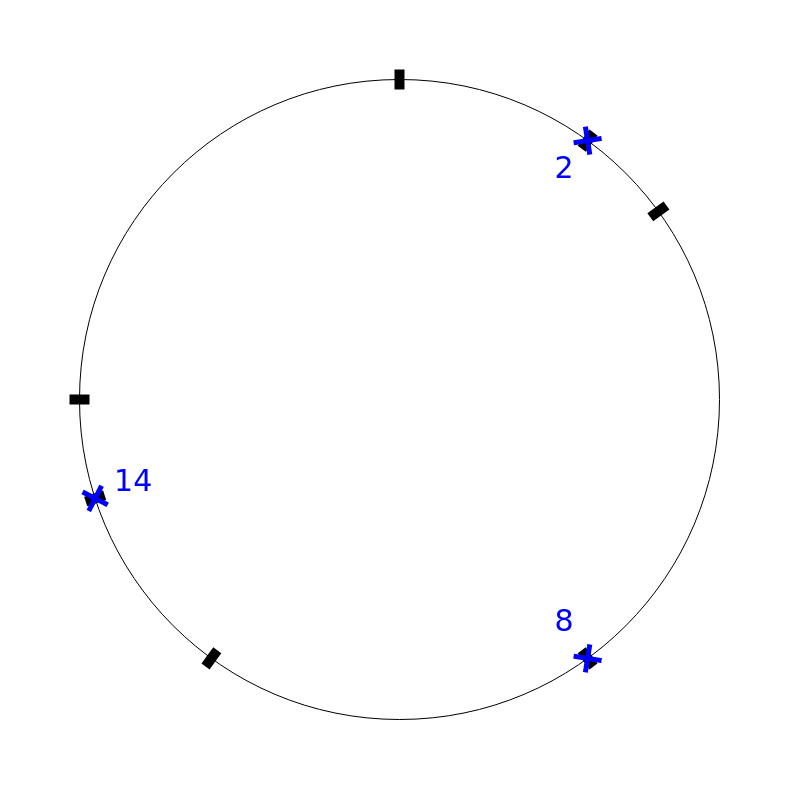
\includegraphics[width=\linewidth]{eisbuden1.png}
        \caption{eisbuden1.txt ($350\mu s$)}
        \label{fig:eisbuden1}
    \end{subfigure}
    \begin{subfigure}[t]{\imageWidth}
        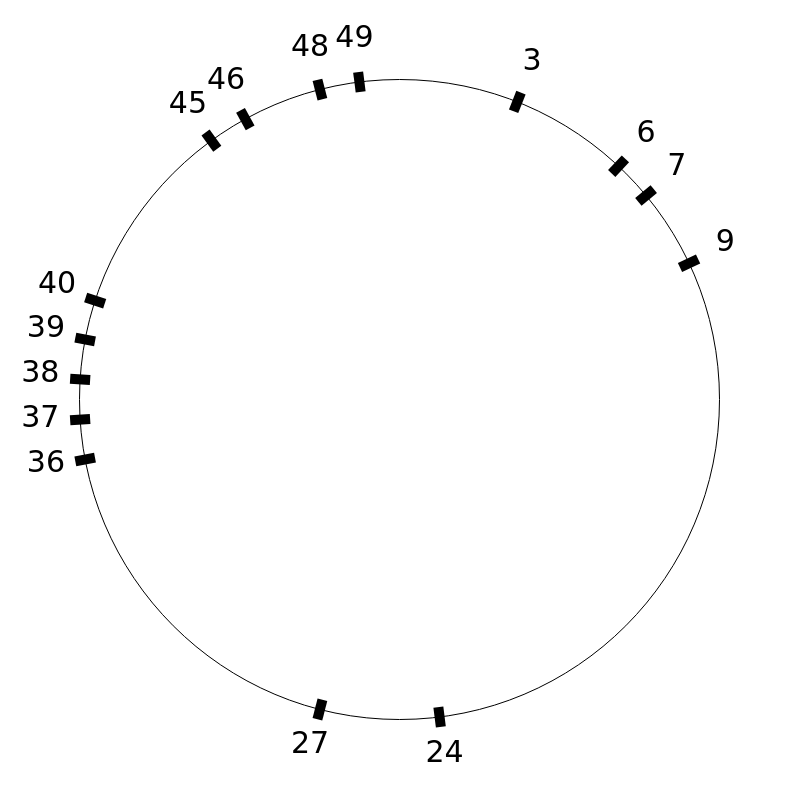
\includegraphics[width=\linewidth]{eisbuden2.png}
        \caption{eisbuden2.txt}
        \label{fig:eisbuden2}
    \end{subfigure}
    \begin{subfigure}[t]{\imageWidth}
        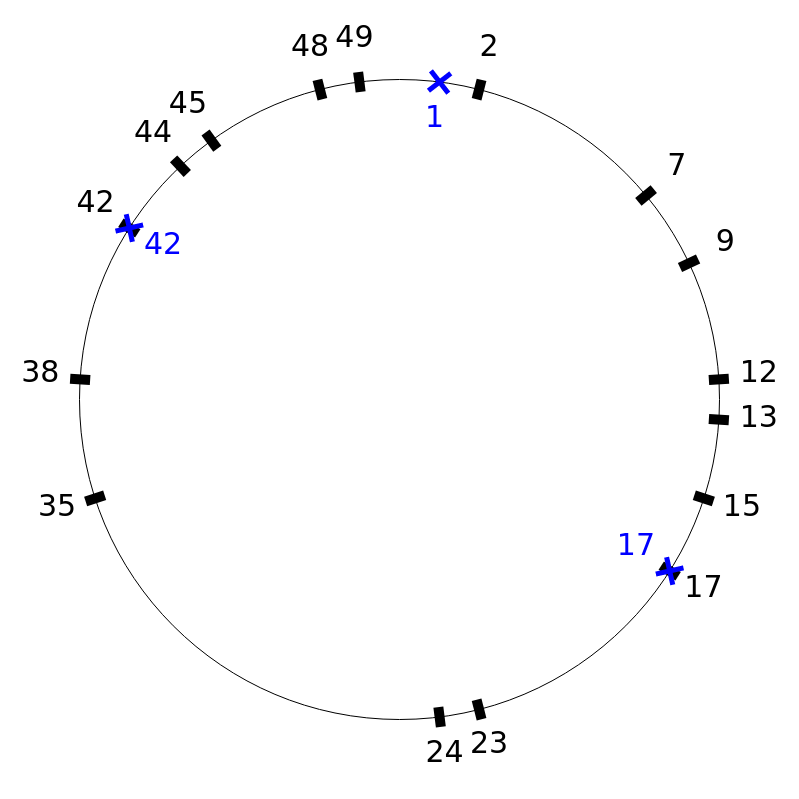
\includegraphics[width=\linewidth]{eisbuden3.png}
        \caption{eisbuden3.txt ($21ms$)}
        \label{fig:eisbuden3}
    \end{subfigure}
    \begin{subfigure}[t]{\imageWidth}
        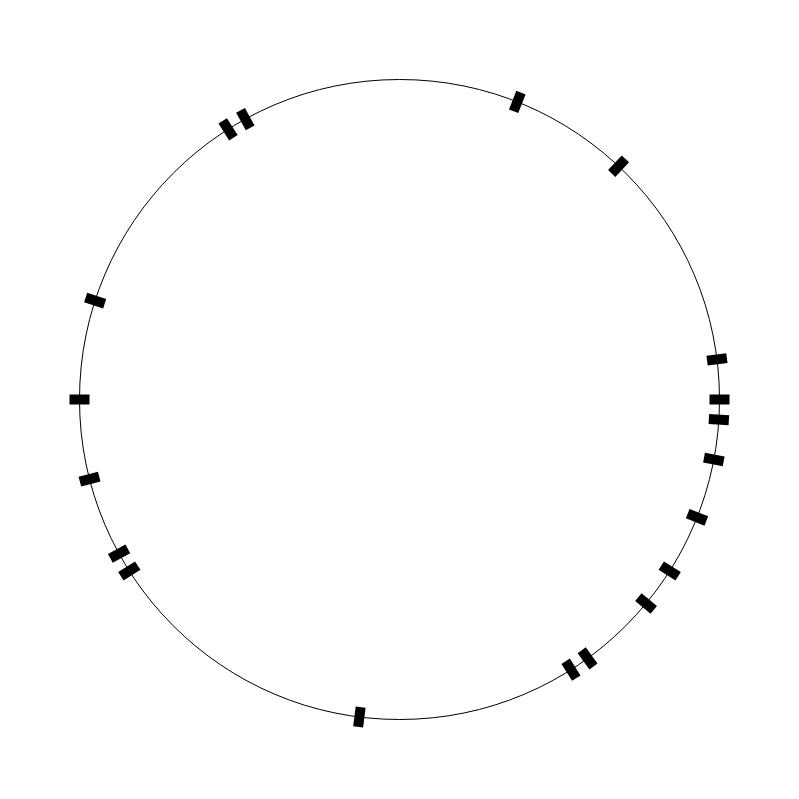
\includegraphics[width=\linewidth]{eisbuden4.png}
        \caption{eisbuden4.txt}
        \label{fig:eisbuden4}
    \end{subfigure}
    \begin{subfigure}[t]{\imageWidth}
        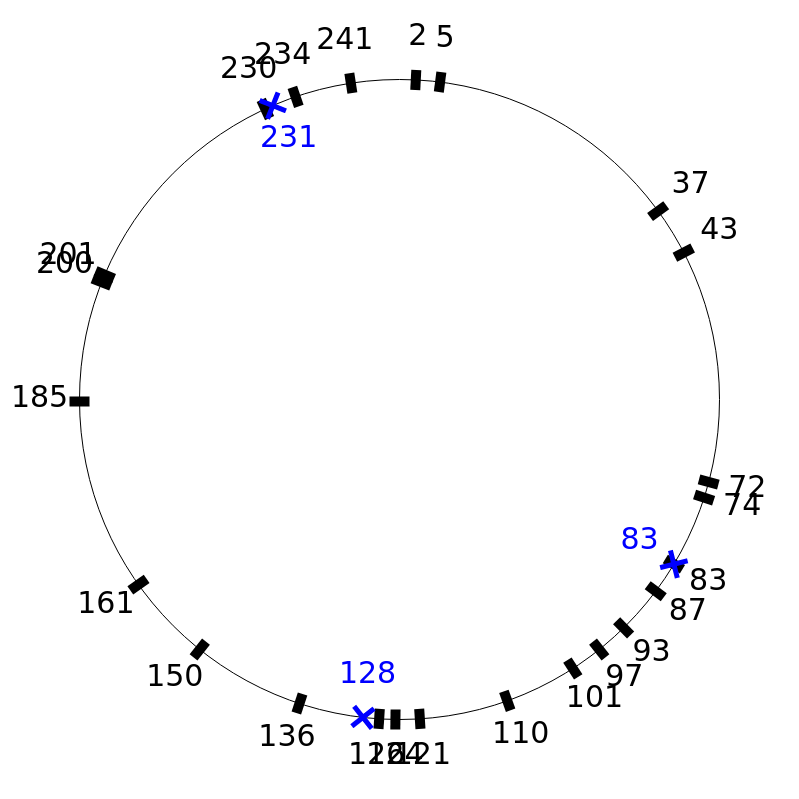
\includegraphics[width=\linewidth]{eisbuden5.png}
        \caption{eisbuden5.txt ($405ms$)}
        \label{fig:eisbuden5}
    \end{subfigure}
    \begin{subfigure}[t]{\imageWidth}
        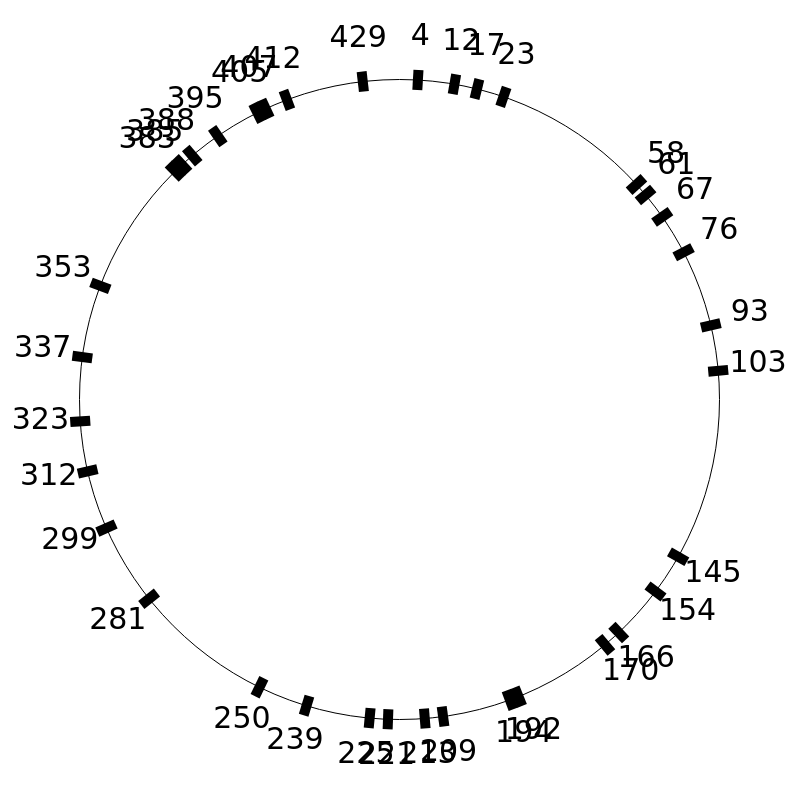
\includegraphics[width=\linewidth]{eisbuden6.png}
        \caption{eisbuden6.txt}
        \label{fig:eisbuden6}
    \end{subfigure}
    \begin{subfigure}[t]{\imageWidth}
        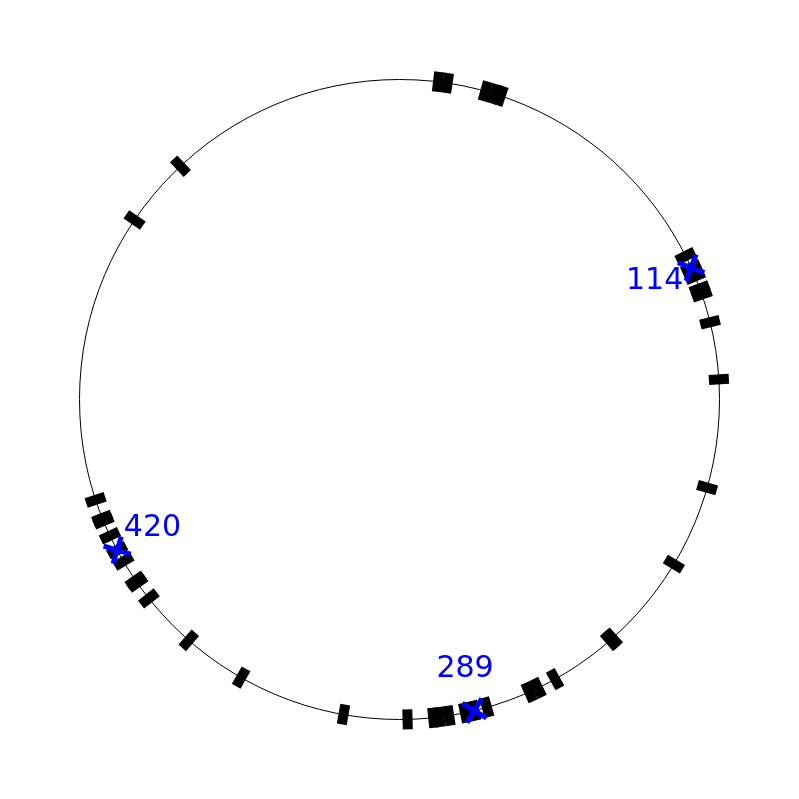
\includegraphics[width=\linewidth]{eisbuden7.png}
        \caption{eisbuden7.txt ($10s$)}
        \label{fig:eisbuden7}
    \end{subfigure}
\end{figure}

\subsection{Eigene Beispiele}
Nun werden einige Grenzfälle mit eigenen Beispielen dargestellt.

\paragraph{myeisbuden0.txt}
Der See dieses Beispiels besitzt einen Umfang von $0$ und keine Häuser.
Dementsprechend geht das Programm davon aus, dass ausschließlich die Adresse 0, die Dorfkirche, existiert.
Daher sind alle möglichen Arrangements \emph{0 0 0}, die alle stabil sind, da kein Haus existiert, das für eine Verlegung stimmen könnte.

Wenn mehr Arrangements getestet werden sollen, als existieren, werden die restlichen Arrangements durch \emph{0 0 0} gefüllt.
Dies ist in einigen Fällen falsch, da dieses Arrangement nicht zwingendermaßen stabil ist.
Zudem führt dies zu der mehrfachen Ausgabe des selben Arrangements.
Eine Überprüfung, ob weniger Arrangements vorliegen als gefordert sind, wurde gewollt nicht implementiert, da
\begin{itemize}
    \item so die Laufzeit verbessert wird,
    \item das Problem nur in Extremfällen vorhanden ist und
    \item es in diesem Fall leicht vom Nutzer erkannt werden kann.
          Dieser kann anschließend manuell die Menge an geforderten Arrangements reduzieren.
\end{itemize}

\paragraph{myeisbuden1.txt}
Dieses Beispiel enthält einen See des Umfangs $100$ und 100 Häuser auf jeder Adresse.
Es ergeben sich genau $400$ stabile Arrangements, unabhängig von der Menge an zu überprüfenden Arrangements.
Der Autor ist davon ausgegangen, dass in diesem Fall alle Arrangements stabil wären, was allerdings bewiesenermaßen nicht der Fall ist.
Zudem ist es bemerkenswert, dass genau $400$ stabile Arrangements eine merkwürdig \glqq glatte\grqq{} Zahl ist.
Wenn diese Datei leicht abgeändert wird und der Umfang des Sees variiert wird, ergebe sich unerwartete Mengen an stabilen Arrangements.
Diese sind in \autoref{tab:Häuser_auf_allen_Adressen} dargestellt.
Eine Begründung für die merkwürdig erscheinenden Mengen wurde nicht gefunden.

\begin{table}[h!t]
    \begin{center}
        \begin{tabularx}{\linewidth}{c|c}
            \textbf{Umfang} & \textbf{Menge stabiler Arrangements} \\
            \midrule
            3               & 1                                    \\
            4               & 4                                    \\
            5               & 10                                   \\
            6               & 20                                   \\
            7               & 14                                   \\
            8               & 32                                   \\
            9               & 21                                   \\
            10              & 40                                   \\
            11              & 22                                   \\
            12              & 52                                   \\
            13              & 26                                   \\
            14              & 56                                   \\
            15              & 35                                   \\
            16              & 64                                   \\
            17              & 34                                   \\
            18              & 78                                   \\
            19              & 38                                   \\
            20              & 80                                   \\
            30              & 130                                  \\
            40              & 160                                  \\
            50              & 200                                  \\
            60              & 260                                  \\
            70              & 280                                  \\
            80              & 320                                  \\
            90              & 390                                  \\
            100             & 400
        \end{tabularx}
        \caption{Seen mit Häusern auf allen Adressen}
        \label{tab:Häuser_auf_allen_Adressen}
    \end{center}
\end{table}

\paragraph{myeisbuden2.txt}
In diesem Beispiel sind drei Häuser gleichmäßig am Rand eines Sees des Umfangs $300$ verteilt.
Es ergeben sich immer nur dann Lösungen, wann zwei Eisdielen auf den Adressen zweier Häuser stehen, da so immer zwei Häuser gegen eine Verlegung stimmen.
Dies ist genug, um diesen Arrangements Stabilität zu verleihen.

\paragraph{myeisbuden3.txt}
Dies ist eine leere Datei, weshalb das Programm mit einer Fehlermeldung abbricht: \glqq File Parsing Error: Not enough elements found!\grqq{}

\paragraph{myeisbuden4.txt}
In diesem Fall wird für den Umfang \glqq aödslkflkja\grqq{} eingesetzt.
Das Programm bricht mit einem Fehler ab: \glqq File Parsing Error: Can't convert "aödslkflkja" to int!\grqq{}

\paragraph{myeisbuden5.txt}
Hier werden den Häusern Adressen gegeben, die für den Umfang zu groß sind.
Das Programm bricht mit einem Fehler ab: \glqq 8 is too big an address for a lake with a circumference of 5!\grqq{}

\section{Quellcode}
% Unwichtige Teile des Programms sollen hier nicht abgedruckt werden. Dieser Teil sollte nicht mehr als 2–3 Seiten umfassen, maximal 10.
Dies ist der Inhalt der Funktion \textbf{is\_stable}.
\begin{lstlisting}
// best routes for test-arrangement
for (int i = 0; i < lake.houses.size(); ++i)
    ice_cream_distances[i] =
        get_ice_cream_distance(lake.circumference, test_arrangement,
                                lake.houses[i]);

// get all other possible locations
// multiple ice cream parlors in same location are a waste
Arrangement check_arrangement;
for (check_arrangement.place_a = 0;
        check_arrangement.place_a < lake.circumference;
        ++check_arrangement.place_a)
    for (check_arrangement.place_b =
                check_arrangement.place_a + 1;
            check_arrangement.place_b <
            lake.circumference;
            ++check_arrangement.place_b)
    {
        // when there are already so many no-votes between place_a and place_b,
        // the location of place_c won't change anything ->
        // this arrangement won't beat the test-arrangement
        if (count_sector_nos(lake, test_arrangement, check_arrangement.place_a,
                                check_arrangement.place_b, false) >= lake.min_nos)
            break;
        // test all possible locations for third ice
        for (check_arrangement.place_c = check_arrangement.place_b + 1;
                check_arrangement.place_c < lake.circumference;
                ++check_arrangement.place_c)
            if (is_better(lake, ice_cream_distances,
                            check_arrangement))
                return false;
        // alternative: calculate nos with count_sector_nos between place_b and
        // place_c, place_c and place_a <- not used <- is actually slower
    }
return true;
\end{lstlisting}

Dies ist der Teil von \textbf{count\_sector\_nos}, der für Release Builds kompiliert wird.
\begin{lstlisting}
int to_right_distance_a = get_abs_distance(lake.circumference, left_side,
    test_arrangement.place_a, Direction::right);
int to_right_distance_b =
    get_abs_distance(lake.circumference, left_side, test_arrangement.place_b,
                        Direction::right);
int to_right_distance_c =
    get_abs_distance(lake.circumference, left_side, test_arrangement.place_c,
                        Direction::right);
// distance from the right to the nearest ice from test-arrangement
int min_to_right_distance = std::min(to_right_distance_a,
    std::min(to_right_distance_b, to_right_distance_c));

// when there is no place from the current arrangement in the sector, all of
// the houses will be delighted to change to the boundaries of the sector ->
// 0 no-votes
int sides_distance = get_abs_distance(lake.circumference, left_side,
                                        right_side, Direction::right);
if (min_to_right_distance >
    sides_distance)
    return 0;

int to_left_distance_a = get_abs_distance(lake.circumference, right_side,
    test_arrangement.place_a, Direction::left);
int to_left_distance_b =
    get_abs_distance(lake.circumference, right_side,
                        test_arrangement.place_b, Direction::left);
int to_left_distance_c =
    get_abs_distance(lake.circumference, right_side,
                        test_arrangement.place_c, Direction::left);

// distance from the left to the nearest ice from test-arrangement
int min_to_left_distance = std::min(to_left_distance_a,
    std::min(to_left_distance_b, to_left_distance_c));

// get borders between which all no-voting houses reside
int left_nos = left_side + (min_to_right_distance + 1) / 2;
int
    right_nos_exclude = right_side - (min_to_left_distance - 1) / 2;

// when the left_middle lays on left_side, it gets moved one to the right <-
// first location in sector doesn't get included; last one does
left_nos += min_to_right_distance == 0;
// when the right_middle lays on right side, it gets moved one to the right
right_nos_exclude += min_to_left_distance == 0;

return count_houses(lake, left_nos, right_nos_exclude);
\end{lstlisting}

\end{document}
